 %We begin by calling the workreport class which includes all the
% definitions for the macros we will use.
\documentclass[ece]{uw-wkrpt}

% We will use some packages to add functionality
\usepackage{graphicx} % Include graphic importing

% Now we will begin writing the document.
\begin{document}

%% First we, should create a title page.  This is done below:
% Fill in the title of your report.
\title{Work Report Title}

% Fill in your name.
\author{First Last}

% Fill in your student ID number.
\uwid{01234567}

% Fill in your home address.
\address{123 Fake Street\\*
         Waterloo, ON\ \ A1B 2CD}

% Fill in your employer's name.
\employer{Company Name}

% Fill in your employer's city and province.
\employeraddress{Waterloo, ON}

% Fill in your school's name.
\school{University of Waterloo}

% Fill in your faculty name.
\faculty{Faculty of Engineering}

% Fill in your e-mail address.
\email{flast123@edu.uwaterloo.ca}

% Fill in your term.
\term{2A}

% Fill in your program.
\program{Mechatronics Engineering}

% Fill in the department chair's name.
\chair{Dr. Dept Chair}

% Fill in the department chair's mailing address.
\chairaddress{MME Department,\\*
              University of Waterloo,\\*
	      Waterloo, ON\ \ N2L 3G1}

% If you are writing a "Confidential 1" report, uncomment the next line.
%\confidential{Confidential-1}

% If you want to specify the date, fill it in here.  If you comment out
% this line, today's date will be substituted.
\date{February 30, 20XX}

% Now, we ask LaTeX to generate the title.
\maketitle

%%%%%%%%%%%%%%%%%%%%%%%%%%%%%%%%%%%%%%%%%%%%%%%%%%%%%%%%%%%%%%%%%%%%%
%% FRONT MATTER
%%%%%%%%%%%%%%%%%%%%%%%%%%%%%%%%%%%%%%%%%%%%%%%%%%%%%%%%%%%%%%%%%%%%%
%% \frontmatter will make the \section commands ignore their numbering,
%% it will also use roman page numbers.
\frontmatter

% After this, we must create a letter of submission.
\begin{letter}
I have just completed my nth work term, following my \theterm{} term.
Please find enclosed my first work term report entitled:
``\thetitle'' for the Software group at \theemployer.  

\end{letter}

% We continue with required sections, such as the Contributions and Summary
\begin{onehalfspacing}


% Next, we need to make a Table of Contents, List of Figures and 
% List of Tables.  You will most likely need to run LaTeX twice to
% get these correct.  The first pass for LaTeX to figure out the
% labels, and the second pass to put in the right references.
\tableofcontents
\listoffigures
\listoftables
\pagebreak

\section{Summary}
This is a report that really does a lot. It explains some cool ideas and I really like to talk about them.
\end{onehalfspacing}
%%%%%%%%%%%%%%%%%%%%%%%%%%%%%%%%%%%%%%%%%%%%%%%%%%%%%%%%%%%%%%%%%%%%%
%% REPORT BODY
%%%%%%%%%%%%%%%%%%%%%%%%%%%%%%%%%%%%%%%%%%%%%%%%%%%%%%%%%%%%%%%%%%%%%
%% \main will make the \section commands numbered again,
%% it will also use arabic page numbers.
\mainmatter

\section{Introduction}\label{sec:intro}
This is such a cool thing! I love \LaTeX{}
\pagebreak 

\section{Sample Tables}
This section mostly is just a table.
    \begin{table}[h]
        \centering
        \caption{A table}
        \label{tab:test}
        \begin{tabular}{ |p{3cm}||p{3cm}|p{3cm}|p{3cm}|  }
         \hline
         \multicolumn{4}{|c|}{Country List} \\
         \hline
         Country Name     or Area Name& ISO ALPHA 2 Code &ISO ALPHA 3 Code&ISO numeric Code\\
         \hline
         Afghanistan   & AF    &AFG&   004\\
         Aland Islands&   AX  & ALA   &248\\
         Albania &AL & ALB&  008\\
         Algeria    &DZ & DZA&  012\\
         American Samoa&   AS  & ASM&016\\
         Andorra& AD  & AND   &020\\
         Angola& AO  & AGO&024\\
         \hline
        \end{tabular}
    \end{table}

\section{Sample Figures}
Figure \ref{fig:knuth} shows Donald Knuth. \cite{ref:donpicture}
\begin{figure}
    \centering
    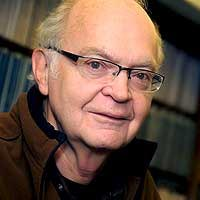
\includegraphics[height=3cm]{test.jpg}
    \caption{Mr. \TeX{} himself \cite{ref:latex2e}}
    \label{fig:knuth}
\end{figure}

\section{TODO}
This is an itemized list of things that need doing in the .cls file.
\begin{itemize}
    \item Numbering of sections $1 \rightarrow 1.0$
\end{itemize}

%%%%%%%%%%%%%%%%%%%%%%%%%%%%%%%%%%%%%%%%%%%%%%%%%%%%%%%%%%%%%%%%%%%%%
%% BACK MATTER
%%%%%%%%%%%%%%%%%%%%%%%%%%%%%%%%%%%%%%%%%%%%%%%%%%%%%%%%%%%%%%%%%%%%%
\backmatter

\bibliography{sample-bib}

%%%%%%%%%%%%%%%%%%%%%%%%%%%%%%%%%%%%%%%%%%%%%%%%%%%%%%%%%%%%%%%%%%%%%
%% APPENDICES
%%%%%%%%%%%%%%%%%%%%%%%%%%%%%%%%%%%%%%%%%%%%%%%%%%%%%%%%%%%%%%%%%%%%%
%% \appendix will reset \section numbers and turn them into letters.
%%
%% Don't forget to refer to all your appendices in the main report.
\appendix

\section{Test}\label{app:test}
This is a test appendix. It has a label and everything.

\end{singlespacing}

\end{document}
